\section{Virtual File System (VFS)}
\label{sec:vfs}

\subsection{Lerninhalt}

\begin{itemize}
   \item Sie kennen den Aufbau des Linux-Dateisystems
   \item Sie kennen den Standard \emph{FHS}
   \item Sie kennen virtuelle Dateien, Verzeichnisse und Dateisysteme
   \item Sie kennen das \emph{procfs}-Filesystem
   \item Sie kennen \emph{devfs} und \emph{udev}
   \item Sie kennen \emph{sysfs}-Filesystem
\end{itemize}

\subsection{Filesystem Hierarchy Standard}

\keyword{Linux-Distributionen} besitzen eine spezifischen Struktur, wie Ordner und Datei
im Dateisystem abgelegt sind. Die \keyword{Linux-Foundation} hat diesen Standard mit dem
Namen \keyword{Filesystem Hierarchy Standard (FHS)}\footnote{\url{http://www.linuxfoundation.org/collaborate/workgroups/lsb/fhs}} erarbeitet, damit Linux- und 
Unix-Devirate kompatibel zueinander sind. Die Abbildung \ref{fig:vfs_structure} zeigt die wichtigsten Verzechnisse des FHS auf.

\begin{figure}[h!]
   \begin{center}
      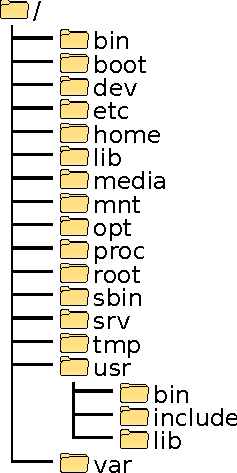
\includegraphics{images/vfs_structure}
   \end{center}
   \caption{Auszug des Filesystem Hierarchy Standard}
   \label{fig:vfs_structure}
\end{figure}

\begin{center}
   \begin{longtable}{| l | p{12cm} |} \hline
      \textbf{Verzeichnis} & \textbf{Beschreibung} \\ \hline 
      / & Das Root-Verzeichnis, welches alle anderen Ordner und Dateien beinhaltet. \\ \hline 
      /bin &  Wesentliche Programme, die auch im \keyword{Single-User-Mode} verfügbar sein müssen. Beispiele: \emph{ls}, \emph{cat}, \emph{cp} \\ \hline 
      /boot & Dateien, die während des Bootprozess gebraucht werden. Hier sind der Linux-Kernel und der Bootloader zu finden. \\ \hline 
      /dev &  Alle Dateien, welche Geräte representieren. In Unix-System werden Geräte über Dateioperationen angesprochen. \\ \hline 
      /etc &  Beinhaltet die Konfigurationsdateien. \\ \hline 
      /home & Alle Benutzerverzeichnisse sind hier zu finden (z.B. \emph{/home/tux}).  \\ \hline 
      /lib &  \keyword{Libaries} für Programme unter \emph{/bin} und \emph{/sbin}. \\ \hline 
      /media & Mit \emph{mount} verbundene Wechseldatenträger (z.B. \emph{CD-ROM}, \emph{USB-Stick}).   \\ \hline 
      /mnt &  Temporär mit \emph{mount} verbundene Datenträger. \\ \hline 
      /opt &  Zusätzliche Software, welche nicht über den \keyword{Packetmanager} installiert wurde. \\ \hline 
      /proc & Informationen über Prozesse und teilweise auch über den Kernel. \\ \hline 
      /root &  Benutzerverzeichnis für den Root-Benutzer.\\ \hline 
      /sbin & Systemprogramme wie \emph{init}. \\ \hline 
      /srv & Dateien, die vom System ausgeliefert werden (z.B. von einem \keyword{Webserver}). \\ \hline 
      /tmp & Temporäre Dateien, welche ohne das ein Datenverlust entsteht gelöscht werden können. \\ \hline 
      /usr & Beinhaltet Dateien für Benutzerprogamme.\\ \hline 
      /usr/bin & Ausführbare Dateien der Benutzerprogramme.  \\ \hline 
      /usr/include & C-Header Dateien für Libraries unter \emph{/usr/lib}.  \\ \hline 
      /usr/lib & Libaries für Programme unter \emph{/usr/bin}. \\ \hline 
      /var & Oft beschriebene Dateien (z.B. Logdatein).  \\ \hline 
      \caption{Übersicht des Dateisystem unter Linux} \\
   \end{longtable}
\end{center}

\subsection{Virtuelle Datei}

Der Linux-Kernel erzeugt, zusätzlich zu den normalen Dateien, auch \keyword[Virtual file]{virtuelle Dateien}. Virtuelle 
Dateien sind auf keinem Datenträger gespeichert, jedoch kann man auf diese Dateien mit den üblichen Dateiopertionen
zugreifen (z.B. \emph{fopen()}, \emph{fread()} und \emph{fwrite()}). Dieser Mechanismus ermöglicht einen Informationsaustausch
zwischen dem Kernel und den Userspace-Programmen und wird \keyword{Virtual Filesystem (VFS)} genannt. \\

Die Verzeichnisse \emph{/proc}, \emph{/dev} und \emph{/sys} unter Linux beinhalten solche virtuelle
Dateien. Die Programme \emph{ps} und \emph{top} erhalten zum Beispiel die Prozessinformationen, wie die CPU-Auslastung und Speicherbelegung, indem
sie bestimmte virtuelle Dateien unter \emph{/proc} auslesen. Um einen Datenträger zu partitonieren schreibt das Programm 
\emph{fdisk} direkt in eine virtuelle Datei unter \emph{/dev}, welche den Datenträger representiert. \\

\subsection{Virtuelles Dateisystem}

Die Verzeichnissse \emph{/proc}, \emph{/dev} und \emph{/sys} sind keineswegs fest an ihren Pfad gebunden. Für diese Verzeichnisse sind die Dateisysteme \keyword{procfs},
\emph{devtmpfs} und \emph{sysfs} zuständig. Sie sind auf dieselbe Weise implementiert wie Dateisysteme für Datenträger (z.B. \keyword{ext2}, \keyword{FAT}), mit dem Unterschied,
dass die Dateien nur im Arbeitsspeicher vorhanden sind. \\

Die virtuellen Dateisysteme werden beim Boot an die jeweillige Stelle gebunden. Der Befehl zeigt alle verbundenen Dateisysteme 
auf, wie das Listing \ref{mounts} zeigt.


\begin{lstlisting}[label=mounts,caption=mount]
$ mount
sysfs on /sys type sysfs (..)
proc on /proc type proc (..)
udev on /dev type devtmpfs (..)
devpts on /dev/pts type devpts (..)
tmpfs on /run type tmpfs (..)
/dev/sda on / type ext4 (..)
tmpfs on /run/lock type tmpfs (..)
tmpfs on /run/shm type tmpfs (..)
binfmt_misc on /proc/sys/fs/binfmt_misc type binfmt_misc (..)
\end{lstlisting}

\subsection{/proc}

Wie bereits erwähnt enthält das Verzeichnis unter \emph{/proc} die Prozessinformationen. 
Für jeden laufenden Prozess erzeugt der Kernel einen neuen Ordner mit der jeweiligen
\keyword{Process-ID (PID)}. Das heisst, der \keyword{Init-Prozess} ist unter \emph{/proc/1/} 
zu finden. Beim Beenden eines Prozesses wird das Verzeichnis wieder gelöscht. \\

Eine gute Übersicht liefern die Dateien unter \emph{/proc/<pid>/status}. Das Listing \ref{init_info}
zeigt den Status des Init-Prozesses. 

\begin{lstlisting}[label=init_info,caption=/proc/1/status]
cat /proc/1/status
Name: init
State:   S (sleeping)
..
Pid:  1
..
Uid:  0  0  0  0
Gid:  0  0  0  0
..
VmSize:     2284 kB
...
Threads: 1
..
\end{lstlisting}

Über diese Datei lassen sich der Name, den aktuellen Prozessstatus, die PID, die \keyword{User-ID (UID)}, die \keyword{Group-ID (GID)},
die Grösse des virtuellen Speichers (VmSize) und die Anzahl Threads finden. 

\subsubsection{procfs}

Hinter dem \emph{/proc}-Verzeichnis steht das virtuelle Dateisystem \keyword{procfs}. Mit folgendem Befehl kann man dieses an einen beliebigen Ort mounten.
\begin{lstlisting}
mount -t proc proc /path/to/directory
\end{lstlisting}


\subsection{/dev}

Das \emph{/dev}-Verzechnis enthält alle verfügbaren Devices, wie Festplatten, Tastaturen und Bildschirme. Zu Beginn von Unix waren die Geräte statisch erstellt
worden. Es gab somit eine vorgegebene maximale Anzahl von Geräten, die angeschlossen werden konnten. Für Linux, welches vom kleinen Router bis zum Grossrechner
vielfälltig eingesetzt wird, ist das nicht geeignet. \\

Aus diesem Grund wurde das virtuelle Dateisystem \keyword{devfs} erfunden. Es ermöglichte Gerätedateien in \emph{/dev} dynamisch hinzuzufügen und zu entfernen.
Dadurch wurde Linux auch \keyword{Plug'n'Play} fähig. Der Nachteil an \emph{devfs} ist jedoch, dass die Namen der Gerätedatei nur vom Kernel festgelegt werden
können. Folglich werden zum Beispiel alle \keyword{SCSI}-Datenträger unter \emph{/dev/sdX} erstellt, wobei mit X die Datenträger alphabetisch nummeriert werden. \\

Deshalb wurde seit ungefähr Kernel 2.6.32 \keyword{udev} entwickelt. \emph{udev} ist ein Daemon-Programm, welches Nachrichten über \keyword[uevent]{uevents} erhält 
und die Dateien in \emph{/dev} erstellt. In \emph{/etc/udev/rules.d/} können eigene Regeln erstellt werden, wie Gerätedateien benannt werden sollen.

\subsubsection{uevent}

Die \emph{uevents} sind Nachrichten vom Kernel an Userspace-Programme. Sie können über \keyword{Netlink}-Sockets empfangen. Netlink-Socket können auf die gleiche Weise
wie \keyword{TCP}- oder \keyword{UDP}-Sockets unter Linux geöffnet werden. Mit folgendem Aufruf kann ein solcher Socket erstellt werden.
\begin{lstlisting}
int sockfd = socket(PF_NETLINK, SOCK_DGRAM, NETLINK_KOBJECT_UEVENT);
\end{lstlisting}

\subsection{/sys}

Relativ neu im Kernel ist das \emph{/sys}-Verzeichnis. Es wurde geschaffen um Informationen über Geräte zu strukturieren. Bis anhin wurden Namen, Seriennummern, Featuresunterstützung 
und weitere Informationen über die Geräte je nach Typ unterschiedlich in \emph{/proc} erfasst. Das war umständlich und stellte einen Missbrauch des \emph{/proc}-Verzeichnisses dar, welches
im eigentlichen Sinne nur für Prozessinformationen gedacht ist. Hinter dem \emph{/sys}-Verzeichnis steckt das virtuelle Dateisystem \keyword{sysfs}.

\subsubsection{sysfs}

Dateien und Ornder in \emph{sysfs} müssen gewisse Regel befolgen, um im Mainline-Kernel aufgenommen zu werden. So darf eine Datei nur einen Wert beinhalten (z.B. ein Integerwert).
Desweiteren sieht der Aufbau die Verzeichnisse \emph{block}, \emph{bus}, \emph{class}, \emph{devices}, \emph{firmware}, \emph{module}, \emph{power} vor, wie Abbildung \ref{fig:sysfs}
zeigt.

\begin{figure}[h!]
   \begin{center}
      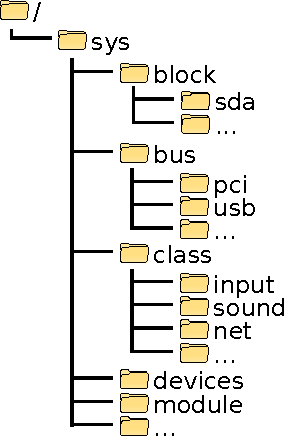
\includegraphics{images/sysfs}
   \end{center}
   \caption{Struktur von Sysfs}
   \label{fig:sysfs}
\end{figure}

\begin{description}
   \item[block] Alle gefundenen Blockgeräte werden hier aufgelistet. Blockgeräte sind meistens Datenträger, bezeichnen aber alle Geräte die Blockweise an einer beliebigen Stelle gelesen werden können.
   \item[bus] Eine Liste mit den aktiven Bus-Systemen. Pro Bus sind wiederum die Geräte, die an diesem Bus gefunden werden, verlinkt.
   \item[class] Alle Geräte sortiert nach der jeweiligen Klasse. Eine Klasse definiert ein Set von Funktionsaufrufen, die für diese Geräte erlaubt sind (z.B. Netwerk- oder Blockgeräteklasse).
   \item[devices] Alle Geräte und Busse hierachisch geordnet, wie sie im System physikalisch vorkommen.
   \item[module] Beinhaltet alle geladenen Kernel-Module.
\end{description}

\subsection{Zusammenfassung}

\begin{itemize}
   \item Sie kennen den Aufbau des Linux-Dateisystems
   \item Sie kennen den Standard \emph{FHS}
   \item Sie kennen virtuelle Dateien, Verzeichnisse und Dateisysteme
   \item Sie kennen das \emph{procfs}-Filesystem
   \item Sie kennen \emph{devfs} und \emph{udev}
   \item Sie kennen \emph{Sysfs}-Filesystem
\end{itemize}

\summary{
Der Filesystem Hierarchy Standard (FHS) wurde von der Linux Foundation entwickelt, um die Unix-Systeme kompatibel zu halten. \\

Eine virtuelle Datei ist nicht physikalisch auf einem Datenträger vorhanden. Sie dient zur Interaktion zwichen Userspace-Programmen
und dem Kernel. \\

Virtuelle Dateisysteme können mit mount verbunden werden wie normale Dateisysteme (ext2, fat, etc.). Beispiele für virtuelle
Dateisysteme sind procfs, devfs und sysfs. \\

Procfs beinhaltet Informationen über Prozesse und weitere Kernelinterne Informationen. \\

Udev löste devfs ab und ist verantwortlich für die Auflistung der Geräte unter /dev. \\

Sysfs wurde entwickelt um Kernel-Informationen struktiert dem Userspace zur Verfügung zu stellen, damit dafür nicht das procfs
missbraucht werden muss.
}

\subsection{Diskussion}

\begin{itemize}
   \item Aus welchem Grund ist ein Standard wie FHS überhaupt sinnvoll?
   \item Wie kann ein Gerät (z.B. Tastatur) als Datei representiert werden?
   \item Wofür sind virtuelle Dateien gut?
   \item Wo wird das \emph{/proc}-Verzeichnis beim Boot gemountet?
   \item Von welchem Datenträger unter \emph{/dev} wurde das System gebootet? Wie kann man das herausfinden?
   \item Das \emph{/sys}-Verzeichnis ist kein Bestandteil von FHS. Ist Linux deshalb überhaupt kompatibel mit dem Standard?
\end{itemize}

